\begin{figure*}[t]
    \centering
    \setlength{\abovecaptionskip}{2mm}
    \centering
    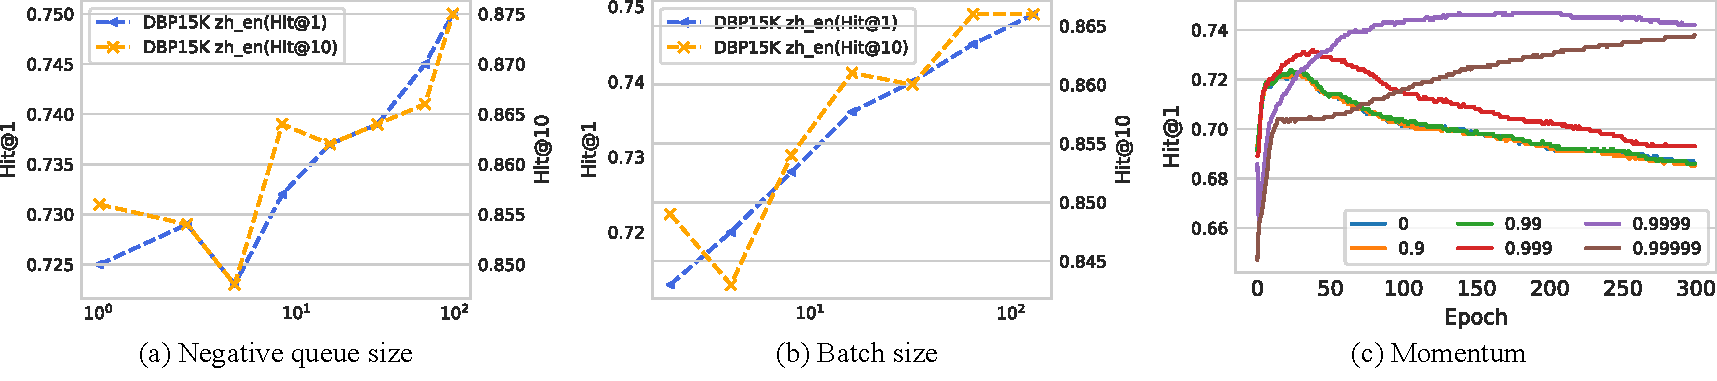
\includegraphics[width=.98\linewidth]{img/selfkg_ablation.pdf}
    \caption{Study on (a) negative queue size, (b) batch size, and (c) momentum on DBP15K$_{\text{zh\_en}}$. (c) presents the test Hit@1 curve throughout the training epochs.}
    \label{fig:size_study}
    %\vspace{-2mm}
\end{figure*}

\begin{figure}
    \centering
        \setlength{\abovecaptionskip}{2mm}
        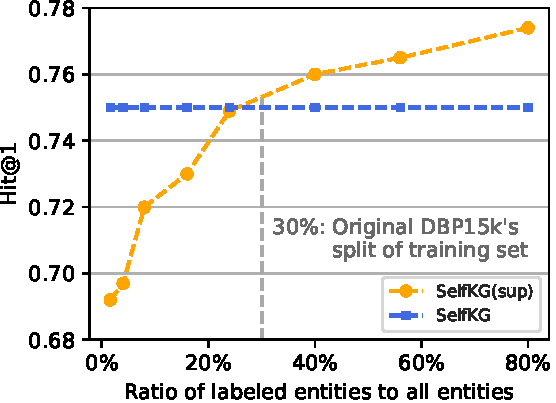
\includegraphics[width=0.9\linewidth]{img/sup.pdf}
        \caption{\solution vs. \solution(sup) on DBP15K. \textmd{\solution works well in a low-data resource setting.}}
        \label{fig:sup}
        \vspace{-0.4cm}
\end{figure}
% \solution is approximately comparable to its supervised counterpart using 90\% of the original training set.